\documentclass[11pt]{article}


\usepackage[a4paper,
            mag=1000, includefoot,
            left=3cm, right=1.5cm, top=2cm, bottom=2cm, headsep=1cm, footskip=1cm]{geometry}

% \linespread{1.5}
% \allowdisplaybreaks[4]o

%\documentclass[11pt]{article}
\usepackage[utf8]{inputenc}
%\usepackage[english]{babel}
\usepackage{graphicx}
%\usepackage{caption}
\usepackage[table,xcdraw]{xcolor}
\usepackage{epigraph}
\usepackage{float}

%\usepackage{amssymb}
%\usepackage{amsmath}
%%

\usepackage{latexsym,amssymb,amsthm}
\usepackage{amsfonts}
%\usepackage[T2A]{fontenc}
\usepackage{amsmath}
\usepackage{url}
\usepackage{pgfplots}

\usepackage{indentfirst}

%\usepackage{refcheck} 


 % \voffset -24.5mm
 % \hoffset -5mm
 % \textwidth 173mm
 % \textheight 240mm
 % \oddsidemargin=0mm \evensidemargin=0mm

\numberwithin{equation}{section}
\newtheorem{theorem}{Theorem}[section]
\newtheorem{lemma}{Lemma}[section]
\newtheorem{proposition}{Proposition}[section]
\theoremstyle{definition}
%\theoremstyle{remark}
\newtheorem{remark}{Note}[section]
\newtheorem{corollary}{Corollary}[section]
\newtheorem{example}{Example}[section]
\newtheorem{definition}{Definition}[section]

\setcounter{tocdepth}{2}

\newcommand{\cov}{\mathrm {cov}}
% \newcommand{\Pr}{\mathrm {Pr}}

\usepackage{color}

\title{A Gentle Introduction to Compressed Sensing}
\author{Andrey V. Bzikadze}

\begin{document}

\maketitle
\epigraph{The \textbf{data deluge} refers to the situation where the volume of new data being generated is overwhelming the capacity of institutions to manage it and researchers to make use of it.}

\section{Introduction}
In the last decade the humanity has come to the point when it produces much more information than it can store and analyse.
There is a huge exposion in the variety of sensors and their dimensionality in many areas: video, audio, scientific, medical research.
Because of that we face the problem of \textbf{data deluge} and naturally come to the necessity of compressing data.

The problem that we will consider can be calculated as follows.
We want to transmit a signal (usually continuous), but we are unable to do it, because the transmission channel is quite narrow.
What strategies can we come up with?

Let us consider the so-called ``Sample-Then-Compress Paradigm'' (Fig~\ref{fig:CSSampleCompressParadigm}).
We sample the signal $n$ times (vector in $\mathbb R^n$).
The transmission channel is narrow, thus, we lossy compress the sample to the dimension $d \ll n$ (vector in $\mathbb R^d$).
Afterwards, the received compressed sample is decompressed to previous dimension $n$ and we try to recover the signal.

This strategy has a number of flaws.
First, how big should $n$ be for us to recover the signal ``well enough'' and is it possible with the limitation of $d$?
Secondly, with $d \ll n$ the process seems somewhat wasteful: why do we actually need $n$ samples if we anyway compress to the dimension $d$?!
Thirdly, at which time points should we measure the signal?
Fourthly, every measurement in the sample could be exorbitant.
Thus, we want to reduce $n$ as much as it is possible.


\begin{figure}[H]
    \begin{center}
        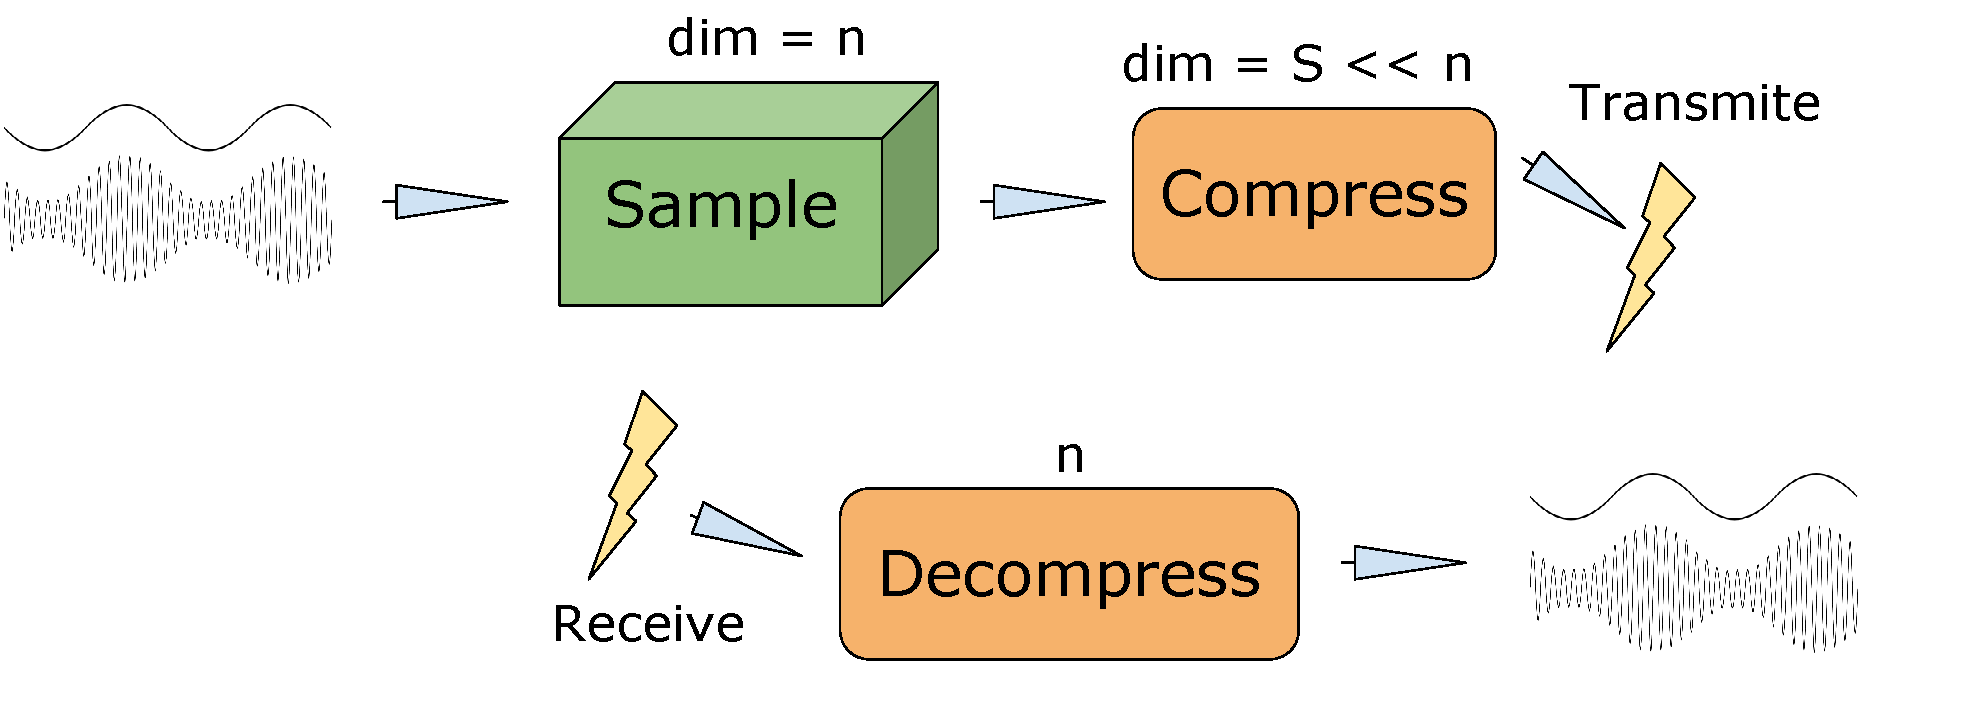
\includegraphics[width=.60\textwidth]{figures/CS_sample_compress_paradigm.pdf}
    \end{center}
    \caption{
        \label{fig:CSSampleCompressParadigm}
        ``Sample-Then-Compress Paradigm''.
        Sample could be a digital camera, a microphone,~\ldots\, Compression strategy is signal-dependent.
    }
\end{figure}

\begin{center}
    \bf \color{red} Maybe we can do better?
\end{center}

\section{Compressed Sensing idea}
\textbf{The first idea of Compressed Sensing} is that the signal at Fig.~\ref{fig:CSSampleCompressParadigm} that we would like to transmit/acquire is often sparse (or ``approximately sparse'') signal in a certain ``basis''.
We will consider a very small example in the section \ref{sec:motivation} that demonstrates that this assumption is feasible.
Suppose that this signal is an $m$-dimensional vector, where $m$ is very large.
Then we want to find a linear basis in $\mathbb R^m$ for this vector to be $S$-sparse (i.e. to have only $S$ nonzero components).
The challenge of the problem is that we do not observe the whole signal.\footnote{
    Suppose that we do.
    Then we can use it as an orth in a basis and the signal is $1$-sparse.
    However, we cannot observe the whole signal because $m$ is very large.
    Take a look at Fig.\ref{fig:CSSampleCompressParadigm}.
    If the signal is an $m$-dimensional vector, then to find the basis we would need to take $n := m$ samples.
    But as we have already discussed we want to reduce $n$ as much as it is possible.
    Because of that we want to find a basis of interest without observing the whole signal.
}

Let us suppose that we now deal with a $S$-sparse signal (we still do not observe it, but know that it is $S$-sparse).
Our aim is to transmit the signal.
\textbf{The second idea of CS} is that we can make measurements that are a certain transformation of the signal.
It means that we can not only measure some distinct components of the $m$-dimensional signal,
but also request, for example, a linear tranformation of the whole signal with some fixed vector.
We want to make as few measurements as possible (to reduce $n$ at Fig.~\ref{fig:CSSampleCompressParadigm}), because each measurement can be expensive.
Without the assumption of us possessing the basis in which the original signal is sparse the problem would have a trivial solution:
we would generally need to make as many measurements as the dimension of a signal.\footnote{Think it through!}
However, the sparsity gives a chance that we need less measurements than the width of the transmission channel $d$
to reconstruct the original signal exactly or approximately.

Generally speaking there are 2 distinct problems:
\begin{itemize}
    \item to find a basis in which the signal is sparse (or approx sparse),
    \item to exactly / approximately reconstruct the signal observing a minimum possible number of measurements.
\end{itemize}
There are theoretical results yielding the minimum number of required measurements needed to produce the original signal given a specific measurement strategy.

In these notes we will not consider the problem of finding the basis in which the signal can be decomposed in a sparse manner.
We will only limit ourselves to a very small example given in the section \ref{sec:motivation}.
Our main concern will be the second problem.

\section{An example of Compressed Sensing sparsity}
\label{sec:motivation}
The main idea of the Compressed Sensing is that a signal vector of our interest is a \textbf{sparse} vector when represented in \textbf{some basis}.
Technically speaking it could be approximately sparse when many components are close to zero.
There are lots of non-formal examples demonstrating this idea, however, many of them are very difficult to formalize.
We will stick to a very simple example that makes a connection with the time series theory.

Let us consider time series $x = \{x_n\}_{n=1}^N$.
The time series $x$ itself is very rarely a sparse vector, i.e. one would not rely on the assumption that $x_n = 0$ for many $n$-s.
However, what could be assumed is that the periodogram has only a few peaks.
Indeed, let us suppose for all $n \in 1:N$
$$ x_n = \sum_{i=1}^S \sin\left(2 \pi w_i \frac{n}{N}\right), $$
where $w_i \in [0, 0.5]$ and $w_i \neq w_j$ for $i \neq j$.
We will suppose that the length $N$ is multiple of the period of $x$.
Then the periodogram will have peaks only at $w_i$.
In this sense the \textbf{Fourier basis} is the basis in which $x$ is $S$-\textbf{sparse}.
Note, that we do not need to know the whole series $x$ to be sure that we possess a basis in which the signal is $S$-sparse.

If with previous assumptions 
$$ x_n = \sum_{i=1}^k \sin\left(2 \pi w_i \frac{n}{N}\right) + \varepsilon_n, $$
for all $n \in 1:N$
where $\varepsilon_n$ is some noise with considerably low variance and zero mean.
Then the periodogram aside possessing peaks at $w_i$ will have small coefficients at the points.
In this sense the \textbf{Fourier basis} is the basis in which $x$ is \textbf{approximately} $S$-\textbf{sparse}.

\section{Problem Statement}
From now on we will only consider the problem of exact or approximate reconstruction of the signal observing a minimum possible number of measurements.

We fix $m \in \mathbb N$. The signal is denoted $\beta^* \in \mathbb R^m$.
We suppose that $\beta^*$ is (strictly) $S$-sparse (has only $S$ non-zero components).
This will be denoted as $\|\beta^*\|_0 = S$.
The $S$ itself is latent (not observed).
We also fix the set of design transformation matrices $\mathbf X_n \in \mathcal M_{n \times m}(\mathbb R)$ for all $n \in \mathbb N$.
The ``measurements'' are denoted $y_n \in \mathbb R^n$ for all $n \in \mathbb N$.
The formal connection between $\beta^*$ and $y_n$ is made through the matrix $\mathbf X_n$ for all $n \in \mathbb N$ and will be explicitly stated.

Let us note one more time that we are aware of $\mathbf X_n$ for all $n$ and observe $y_n$, but do not observe $\beta^*$ and want to find it with the smallest $n$ possible.

\subsection{Noiseless case}
Let us suppose that $y_n = \mathbf X_n \beta^*$ for all $n \in \mathbb N$.
The problem is to obtain $\beta^*$ as the solution of the linear system $y_n = \mathbf X_n \beta$ (the variable $\beta$).
The illustration can be seen at Fig.~\ref{fig:NoiseLessProblemStatement}.
\begin{figure}[H]
    \begin{center}
        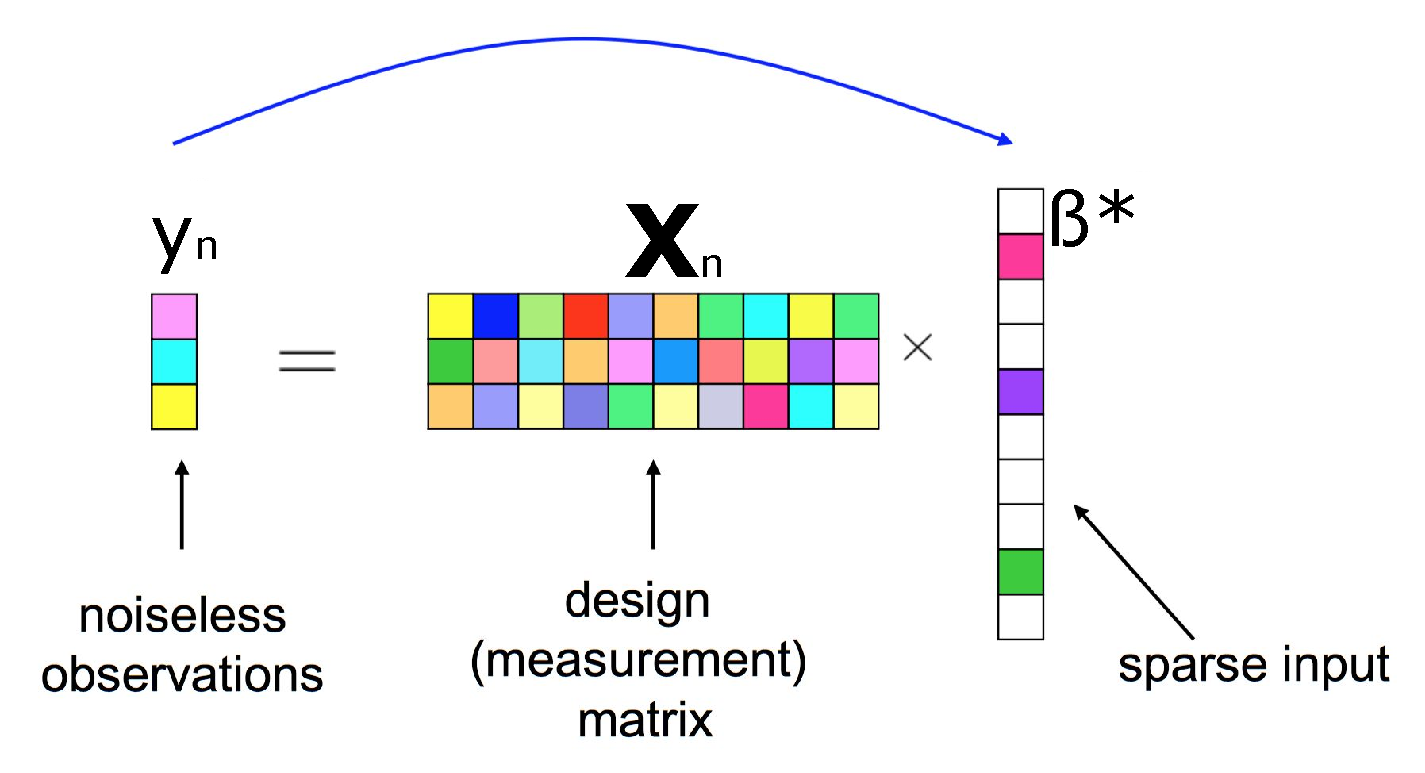
\includegraphics[width=.75\textwidth]{figures/problem_statement_2.pdf}
    \end{center}
    \caption{
        \label{fig:NoiseLessProblemStatement}
        Noiseless problem statement.
    }
\end{figure}

For each $n$ we present the following estimator
\begin{gather}
    \label{eq:noiselessBeta}
    \hat \beta_n = \arg \min_{\beta: y_n = \mathbf X_n \beta} \|\beta\|_1.
\end{gather}

The choice of $n$ such that $\hat \beta = \beta^*$ is heavily influenced by $S$ and $\mathbf X_n$.
We will now consider an example of the family $\{\mathbf X_n\}_{n \geqslant 1}$.

\begin{definition}
    \label{def:rip}
    A matrix $\mathbf A \in \mathcal M_{n, m}(\mathbb R)$ is said to satisfy the \textbf{restricted isometry property} (RIP) of order $S$ with constant $\delta_S$ for $\delta_S \in (0, 1)$ if
    $$ (1 - \delta_S) \|x\|_2^2 \leqslant \|\mathbf A x\|_2^2 \leqslant (1 + \delta_S) \|x\|_2^2 $$
    for all $S$-sparse $x \in \mathbb R^m$.
    
    Notation: $\mathbf A \in \textrm{RIP}(S, \delta_S)$.
\end{definition}

\begin{remark}
    \label{rem:def_rip}
    If we (formally) take $\delta_S = 0$ in the Definition \ref{def:rip} we obtain:
    $$ \|\mathbf A x\|_2^2 = \|x\|_2^2 $$
    for all $S$-sparse $x \in \mathbb R^m$.
    It means that the matrix preserves the norm exactly.

    If we take $\delta_S = 1$:
    $$ 0 \leqslant \|\mathbf A x\|_2^2 \leqslant 2 \|x\|_2^2 $$
    for all $S$-sparse $x \in \mathbb R^m$.
    It means that the matrix can diminish the norm infinitely.

    As a result we can interpret the parameter $\delta_S$ like this: the higher $\delta_S$ is --- the higher the dispersion of $\|\mathbf A x\|_2^2$ is.
\end{remark}

\begin{theorem}
    \label{theorem:CSforRIP}
    Let $\mathbf X_n \in \mathcal M_{n, m} (\mathbb R)$ be $\textrm{RIP}(S, \delta)$ where $S \leq m / 2$ and $\delta \in (0, 1)$. Then for
    $$ n \geqslant C_\delta S \ln(m / S), $$
    where $C_\delta < 1$ is a constant and depends only on $\delta$:
    $$ \hat \beta_n = \beta. $$
\end{theorem}

Proof can be found in Theorem 3.5: \url{mdav.ece.gatech.edu/publications/phdthesis-2010.pdf}.
Let us comment on the result of the theorem.
Suppose, that $S$ is very small comparatively to $m$, then
$$ C_\delta S \ln(m / S) = C_\delta S \ln m - C_\delta S \ln S \approx const \cdot \ln m. $$
It means that we only need to make a number of samples proportional to $\ln m$ instead of $m$ when the assumption about the sparsity is not made.
If $S = m / 2$ then
$$ C_\delta S \ln(m / S) = (C_\delta m \ln 2) / 2 \approx const \cdot m. $$
It means that we need to make a number of samples proportional to $m$.
Consequently, the number of measurements is bounded between $\log m$ and $m$.

The problem of checking the RIP condition for a given matrix is NP-hard.
However, it is easy to simulate a matrix that satisfies RIP with a high probability.

\begin{theorem}
    Fix $\delta \in (0, 1)$.
    Let $\mathbf X_n \in \mathcal M_{n, m} (\mathbb R)$ be a random matrix whose components are independent and have $\mathcal N(0, 1/n^2)$ distribution.
    Fix $C_1 > 0$ such as
    $$ n \geqslant C_1 \ln(m / S), $$
    then 
    $$ \mathbb P(\mathbf X_n \in \textrm{RIP}(S, \delta)) \geq 1 - 2 e^{-C_2 n}, $$
    where $C_2 = C^*\delta^2/2 - \ln (42 e / \delta) / C_1$ and $C^* = 2 / (1 - \ln(2)) \approx 6.52$.
\end{theorem}
Proof can be found in Theorem 4.3: \url{mdav.ece.gatech.edu/publications/phdthesis-2010.pdf}.

\begin{remark}
    Interested people could analyse the constant $C_2$ to find out its dependence on $\delta$.
    Generally, the higher $n$ is --- the higher the probability is.
\end{remark}

\begin{remark}
    Gaussian matrix is very convenient, as to produce it we only need to transfer random seed but not the matrix itself.
\end{remark}

% As we want to make the probability as high as possible, to produce RIP matrix we want $\exp(-C_2n)$ as small as possible.
% It means that $C_2 n$ as large as possible.
% Let's take $C_1$: $n = C_1 \ln(m / S)$:
% $$C_2 n = C_1 C_2 \ln(m / S) = \ln(m / S) [ \delta^2 / 2 - \ln(42 e / \delta) ] = \ln(m/S) [ \delta^2 / 2 + \ln \delta + const ]. $$
% So the probability we are interested in depends on $\delta$: the higher $\delta$ is --- the higher the probability is (with fixed $m$).
% Consider an extreme example of $\delta = 1$:
% $$ \mathbb P(\mathbf X_n \in \textrm{RIP}(S, \delta)) \geq 1 - 2 e^{-C_2 n} = 1 - 2 e^{ \ln{m/S}(0.5 + \ln(42))} \approx 1 - 2 e^{4.2 \ln(m/S)}. $$
% WTF???

Let us note that the RIProperty  is not the only condition that allows to formulate results similar to the theorem \ref{theorem:CSforRIP}.
There are plenty of them, see Section 3.1.3: \url{https://sites.google.com/site/igorcarron2/cs}.
RIP is somewhat the most traditional.

\subsection{Noisy case}
Let us suppose that $y_n = X_n \beta^* + \varepsilon_n$ for all $n \in \mathbb N$, where $\varepsilon_n$ is the noise.
The conditions on it with be formalized further.
The problem is to obtain $\beta^*$ as an approximate solution to the linear system $y_n \approx \mathbf X_n \beta$ (the variable $\beta$).
The illustration can be seen at Fig.~\ref{fig:NoisyProblemStatement}.
\begin{figure}[H]
    \begin{center}
        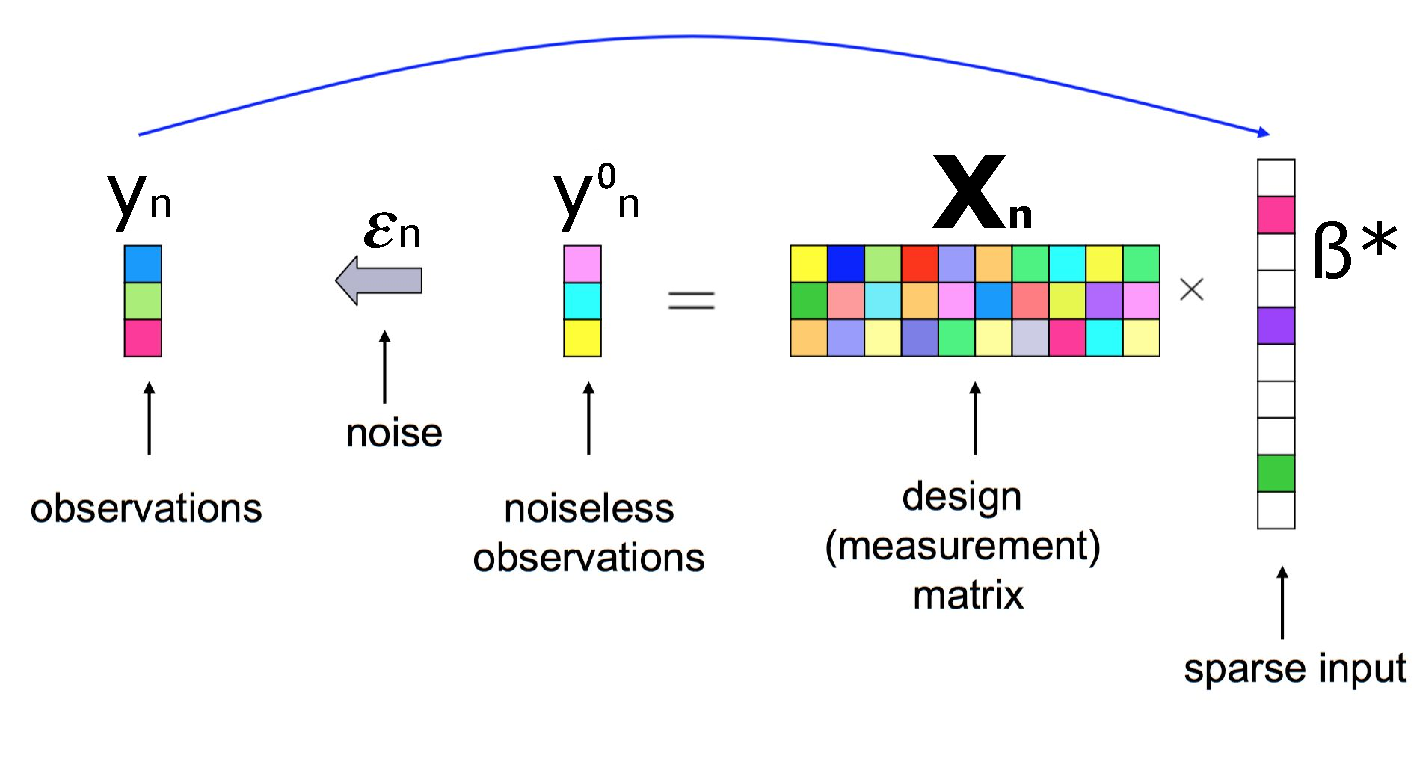
\includegraphics[width=.75\textwidth]{figures/problem_statement_3_noisy.pdf}
    \end{center}
    \caption{
        \label{fig:NoisyProblemStatement}
        Noisy problem statement.
    }
\end{figure}

For each $n$ and accuracy $\delta > 0$ we present the following estimator
\begin{gather*}
    \hat \beta_n(\delta) = \arg \min_{\beta: \|y_n - \mathbf X_n \beta\|_2^2 \leqslant \delta} \|\beta\|_1.
\end{gather*}

The choice of $n$ such that $\hat \beta \approx \beta^*$ is heavily influenced by $S$ and $\mathbf X_n$.
The results similar to the noiseless case hold here for RIP matrices.

Let us consider the following elaboration on the optimization problem:
$$ \min_{\beta: \|y_n - \mathbf X_n \beta\|_2^2 \leqslant \delta} \|\beta\|_1 $$
is equivalent to LASSO:
$$ \min_{\beta: \|\beta\|_1 \leqslant t} \|y_n - \mathbf X_n \beta\|_2^2 $$
for a certain $t$.
Thus, we can apply the numerical procedures for LASSO problem (LARS).
\begin{remark}
    When talking about the special features of the algorithm implementation,
    one can mention that the problem is connected to LASSO and, thus, all techniques of convex optimization are applicable here.
\end{remark}

\begin{center}
    \color{red}
    The following sections are optional.
\end{center}
\small {
\section{Random Fourier projections (Candes et al., 2006)}

This section is devoted to a special choice of the matrices $\mathbf X_n$.
Formally we change the notation.
Let $\mathcal F$ be the Fourier basis matrix in $\mathbb R^m$, $\mathbb T = 1:m$ --- a set of all time points when the measurements could be conducted, $\Omega \subset \mathbb T$ --- when the measurements are conducted.

Instead of \eqref{eq:noiselessBeta} consider
\begin{gather}
    \hat \beta_n = \arg \min_{\substack{\beta: (\mathcal F \beta^*)_t = (\mathcal F \beta)_t \\ t \in \Omega}} \|\beta\|_1.
\end{gather}
The noisy problem is reformulated analogously.

The fundamental result is the following:
\begin{theorem}
    Let $\beta^* \in \mathbb C^m$, $\|\beta^*\|_0 = S$. Let $\Omega \subset \mathbb T$ be a uniformly selected set of a fixed size $n_\Omega$.
    Fix $B > 0$ --- accuracy.
    If
    $$ n_\Omega \geq C(B) n \ln m, $$
    where $C(B) \asymp 23(B + 1)$ then
    $$ \mathbb P(\hat \beta_n = \beta^*) \geq 1 - \mathcal O(m^{-B}). $$
\end{theorem}

\begin{remark}
    $\Omega \subset \mathbb T$ --- a uniformly selected set of a fixed size $n_\Omega$ --- is very difficult to simulate.
    However, we can change this condition to the set of Bernoulli trials:
    $$ \Omega: \mathbb P(j \in \Omega) = \tau $$
    and the theorem changes only slightly.
\end{remark}

\section{The Recovery Theorem for arbitrary bases}

\begin{definition}
    Let $\Phi = \{\phi_i\}$ and $\Psi = \{\psi_j\}$ be the bases in $\mathbb R^m$.
    Then the \textbf{coherence} of orthonormal bases $\Phi$ and $\Psi$.
    $$ \mu(\Phi, \Psi) = \sqrt{m} \max_{i, j} |(\phi_i, \psi_j)|. $$
\end{definition}

\begin{remark}
    Two facts about the coherence:
    \begin{enumerate}
        \item $ 1 \leq \mu(\Phi, \Psi) \leq \sqrt m $.
        \item $\mu(\mathcal F, \mathcal F^{-1}) = 1$.
    \end{enumerate}
\end{remark}

\begin{theorem}[Candes and Romberg, 2007]
    Fix $\delta > 0$, $\beta^* \in \mathbb R^m$.
    Choose $\Omega$ uniformly (of a fixed size).

    Consider the solution to the following convex optimization problem:
    $$ \hat \beta = \arg \min_\beta \|\beta\|_1: (\beta^*, \phi_k) = (\phi_k, \Psi \beta), k \in \Omega. $$
    
    If
    $$ |\Omega| \ge C \mu^2(\Phi, \Psi) \|\beta^*\|_0 \ln \frac{m}{\delta} $$
    then
    $$ \mathbb P(\hat \beta = \beta^*) \ge 1 - \delta. $$
\end{theorem}

\begin{remark}
    The following results about the noisy problem are formulated for RIP matrices and will be out of scope.
\end{remark}
}

\end{document}
